\chapter{結果と考察}
共振周波数を変化させるためには、共振器の大きさを変化させる方法と、と内部に誘電体あるいは導体を挿入する方法がある。共振器自体の大きさを変化させて共振周波数を調整する方法では、全ての辺の長さの比を一定にしなければ、内部の電磁場分布が大きく変化してしまい、大きさの変化とともに試料設置位置も変動させる必要が出てくるが試料設置位置を動かすことは現実的ではない。また、全ての方向で大きさの比を保ちながら共振器の大きさを変化させるためにはかなり高度なギミックが必要となり、これも現実的ではない。そのため今回は内部に誘電体を挿入することによって、共振周波数を現象させるという方法で実現を目指す。


\section{誘電体挿入による影響}
まず、誘電体挿入による影響を調べるための検証を行った。

\vspace{10 mm}

\begin{figure}[h]
  \begin{center}
    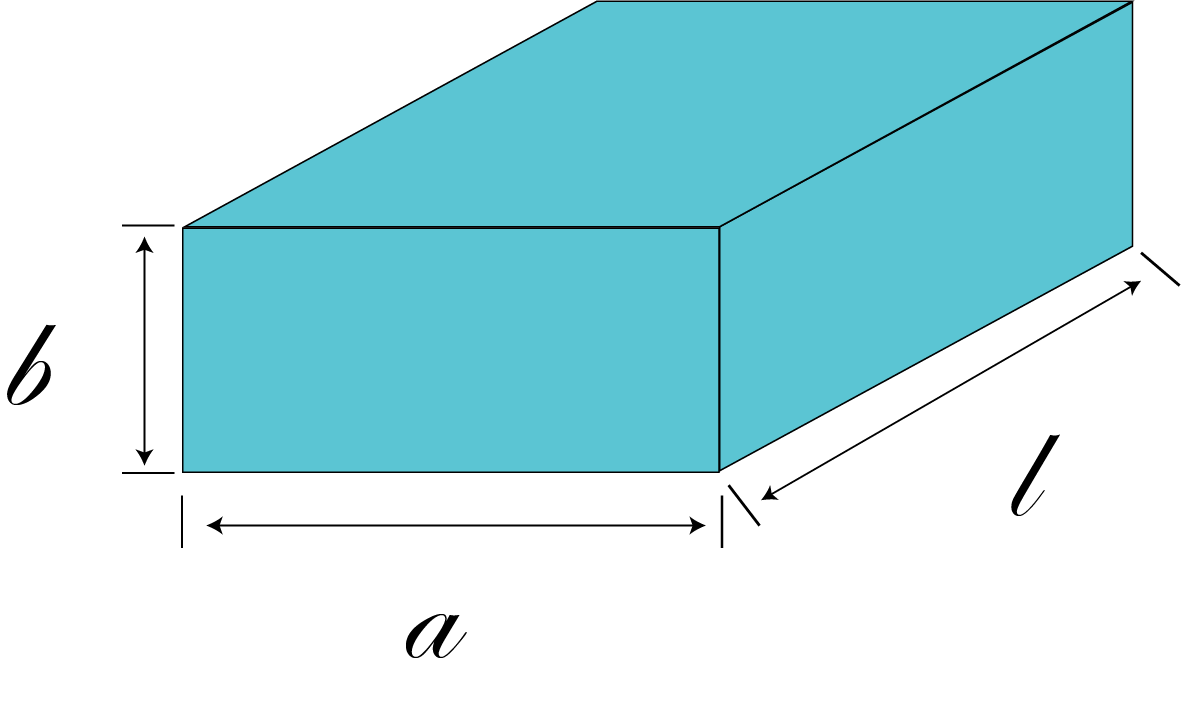
\includegraphics[width=5cm]{./image/空洞共振器.png}
    \caption{TE101の電場分布}
    \label{fig:E-TE101}
  \end{center}
\end{figure}

上図のように基本モード$TE101$を持つ空洞共振器を用いて、誘電率9の誘電体(サファイア)を下図のように

\begin{enumerate}
  \item 共振器よりも小さいサイズで位置のみを変化させたモデル
  \item 共振器と同じサイズで徐々に挿入していくモデル
\end{enumerate}

の2つの場合で検証を行った。

\vspace{10 mm}

\begin{figure}[h]
  \begin{center}
    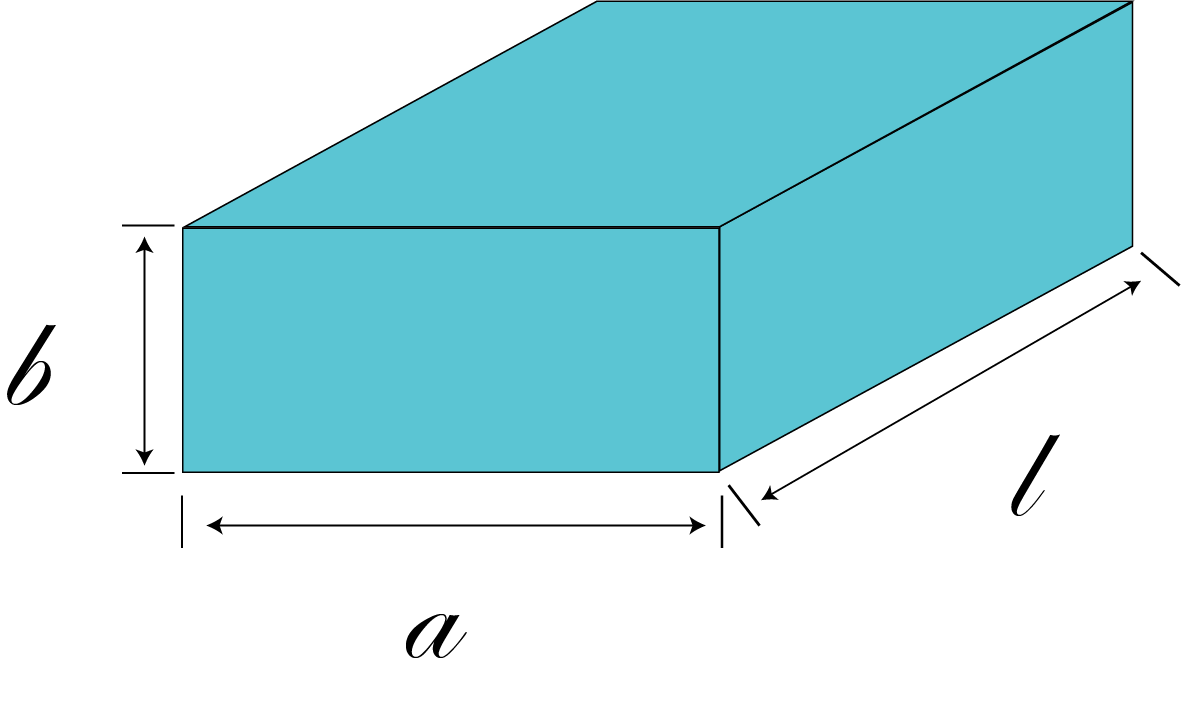
\includegraphics[width=5cm]{./image/空洞共振器.png}
    \caption{位置のみを変化させたモデル}
    \label{fig:potition}
  \end{center}
\end{figure}

\vspace{10 mm}

\begin{figure}[h]
  \begin{center}
    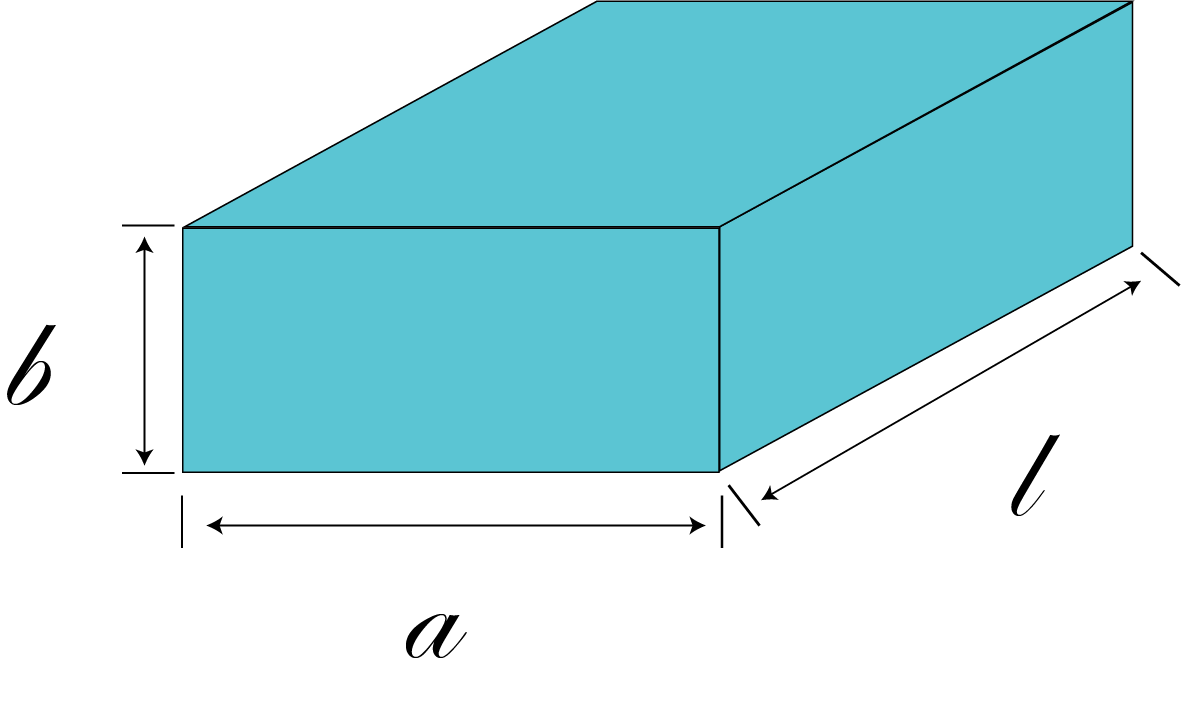
\includegraphics[width=5cm]{./image/空洞共振器.png}
    \caption{誘電体を挿入していったモデル}
    \label{fig:length}
  \end{center}
\end{figure}

\subsection{結果}
結果を以下のグラフに示す。
この結果から、電場振幅の大きい場所に誘電体をおいた方が振幅が小さい場所におくよりも大きく共振周波数が変化すること。また、誘電体の位置だけを変化させる場合と挿入する場合では、変化の最大値は挿入していったモデルの方が大きいということがわかった。


\vspace{10 mm}

\begin{figure}[h]
  \begin{center}
    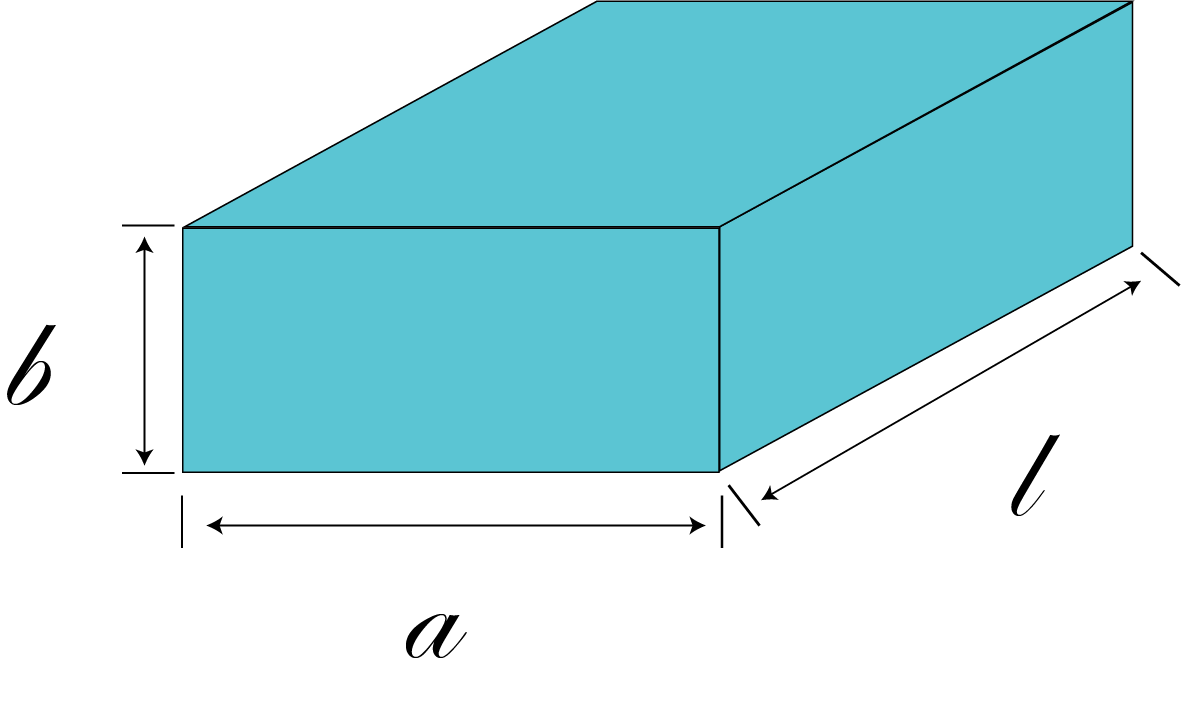
\includegraphics[width=5cm]{./image/空洞共振器.png}
    \caption{誘電体による共振周波数の変化の検証}
    \label{fig:Cavity}
  \end{center}
\end{figure}


\subsection{考察}
これらの結果を受けて、共振周波数を大きく変化させるためには、共振器内部の「電場振幅の大きい場所」に誘電体を「挿入」すると良さそうである。

\section{提案するモデル}
この結果を受けて今回は以下のようなモデルを提案する。
\subsection{設計}


\vspace{10 mm}

\begin{figure}[h]
  \begin{center}
    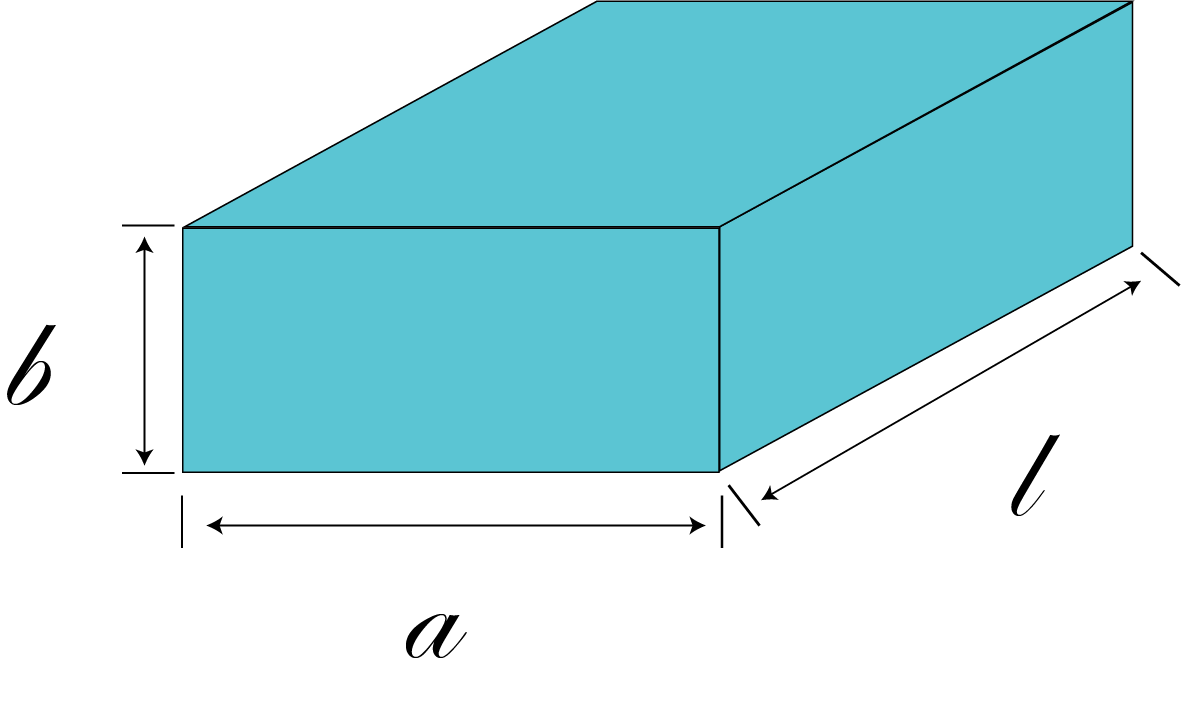
\includegraphics[width=5cm]{./image/空洞共振器.png}
    \caption{方形空洞共振器}
    \label{fig:Cavity}
  \end{center}
\end{figure}

\vspace{10 mm}

\begin{figure}[h]
  \begin{center}
    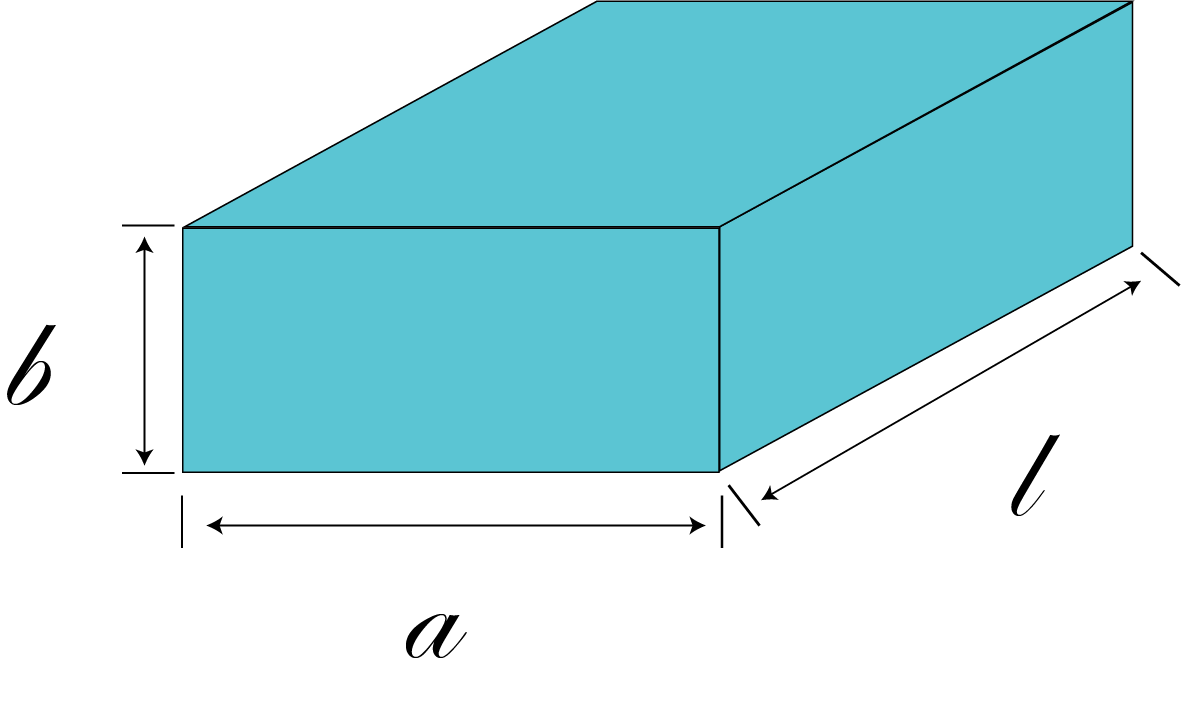
\includegraphics[width=5cm]{./image/空洞共振器.png}
    \caption{方形空洞共振器}
    \label{fig:Cavity}
  \end{center}
\end{figure}

\vspace{10 mm}

\begin{figure}[h]
  \begin{center}
    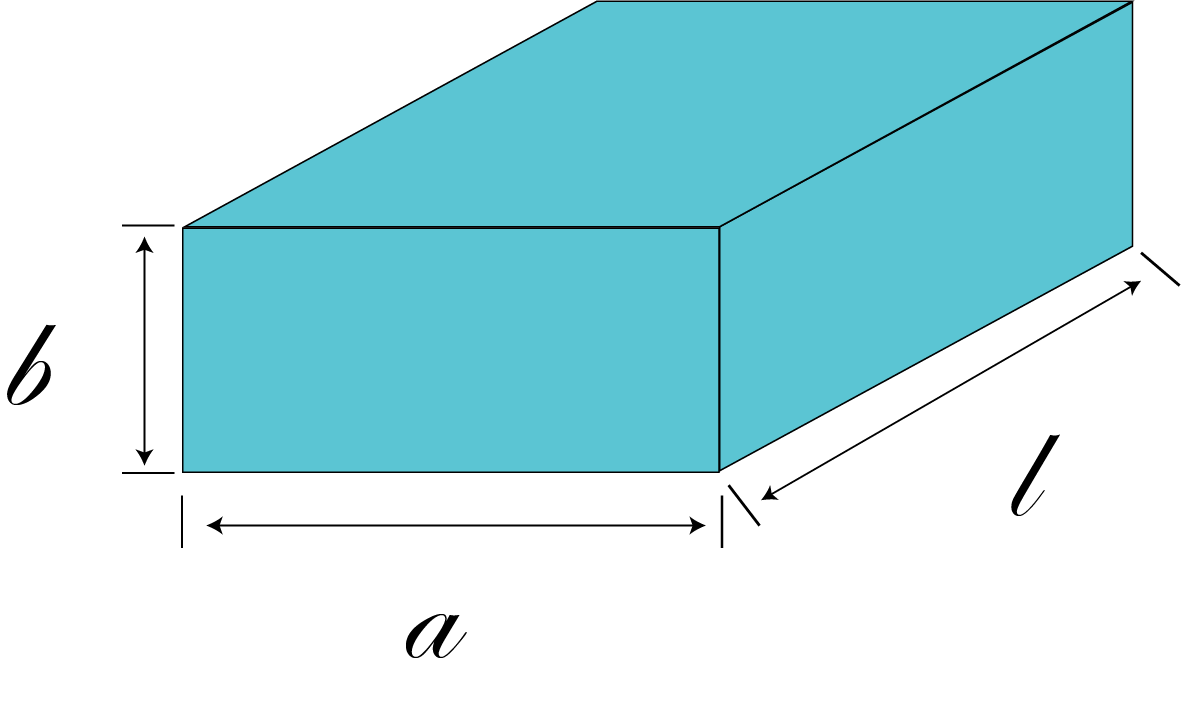
\includegraphics[width=5cm]{./image/空洞共振器.png}
    \caption{方形空洞共振器}
    \label{fig:Cavity}
  \end{center}
\end{figure}

\vspace{10 mm}

\begin{figure}[h]
  \begin{center}
    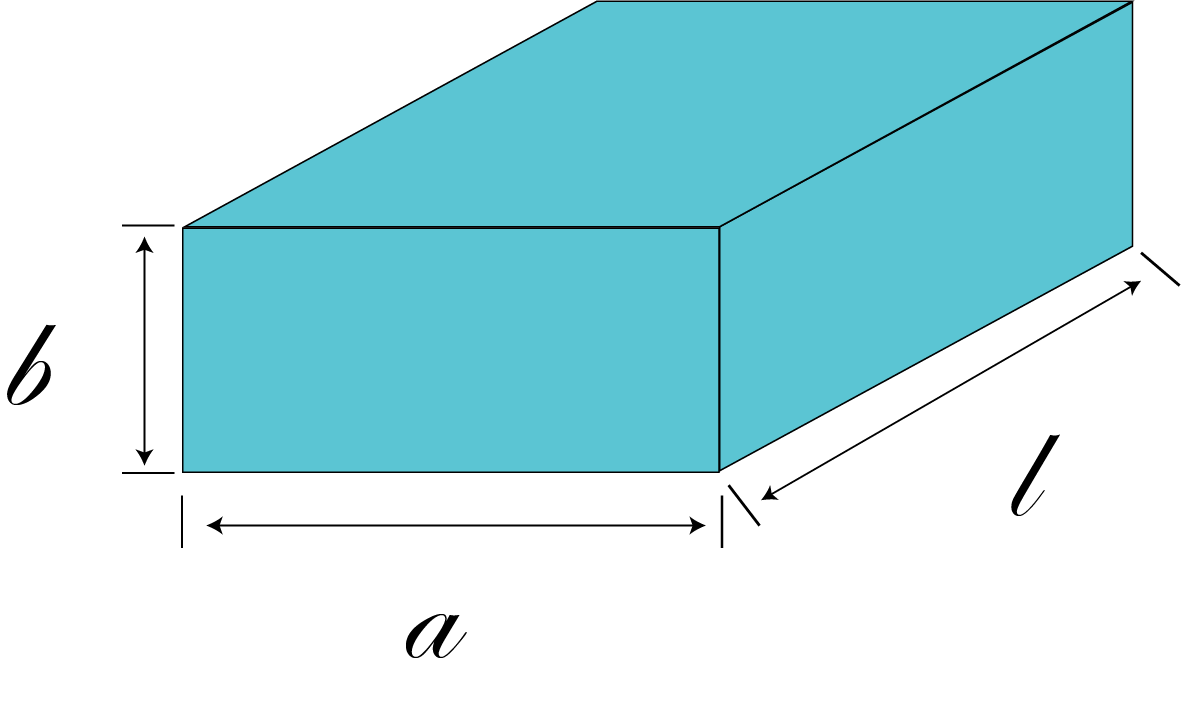
\includegraphics[width=5cm]{./image/空洞共振器.png}
    \caption{方形空洞共振器}
    \label{fig:Cavity}
  \end{center}
\end{figure}

\subsection{基本性質}
\vspace{10 mm}

\begin{figure}[h]
  \begin{center}
    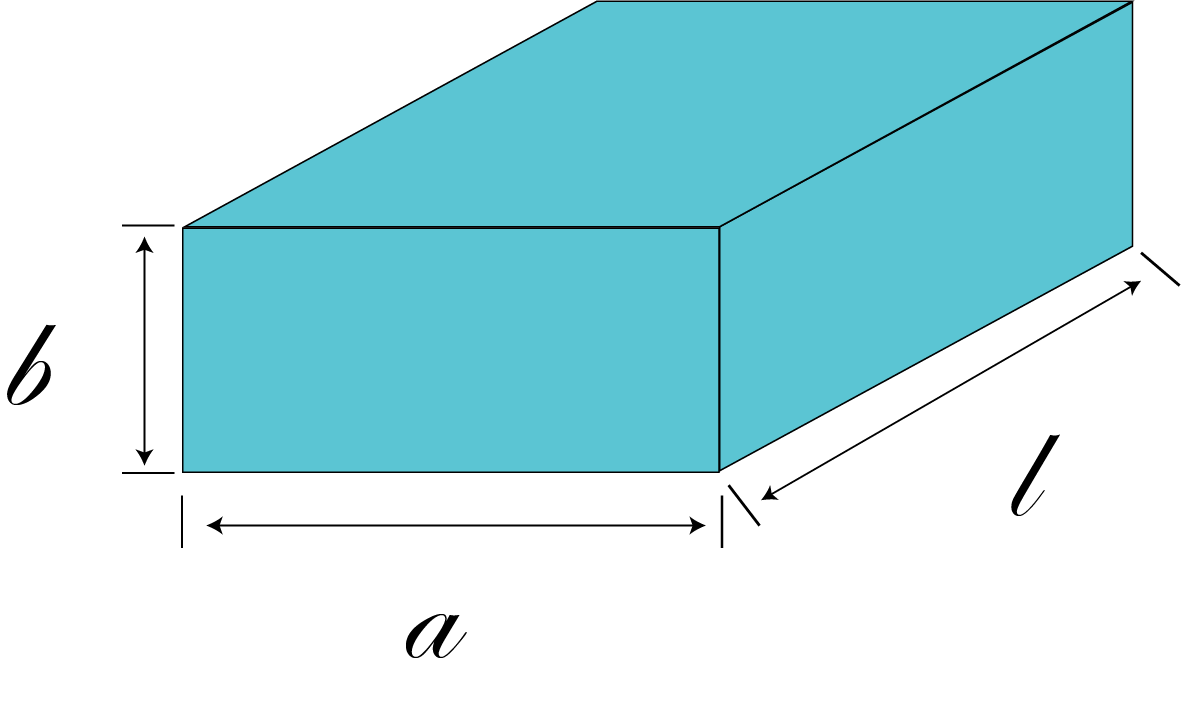
\includegraphics[width=5cm]{./image/空洞共振器.png}
    \caption{方形空洞共振器}
    \label{fig:Cavity}
  \end{center}
\end{figure}

\vspace{10 mm}

\begin{figure}[h]
  \begin{center}
    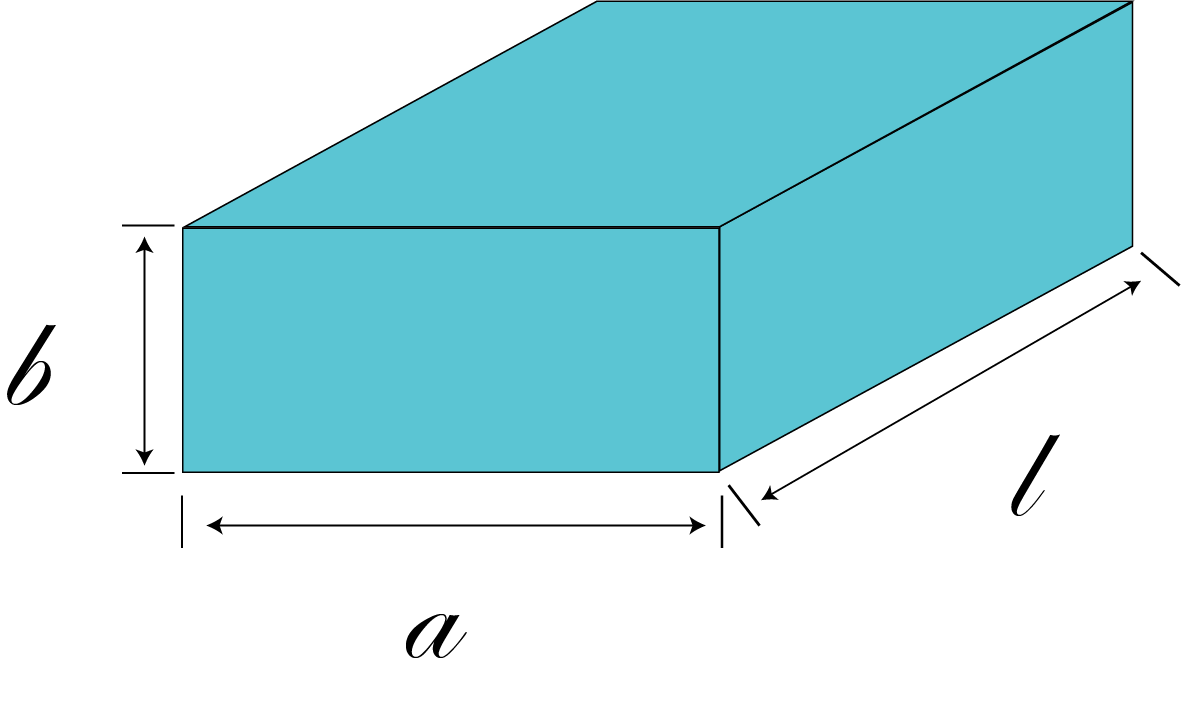
\includegraphics[width=5cm]{./image/空洞共振器.png}
    \caption{方形空洞共振器}
    \label{fig:Cavity}
  \end{center}
\end{figure}

\vspace{10 mm}

\begin{figure}[h]
  \begin{center}
    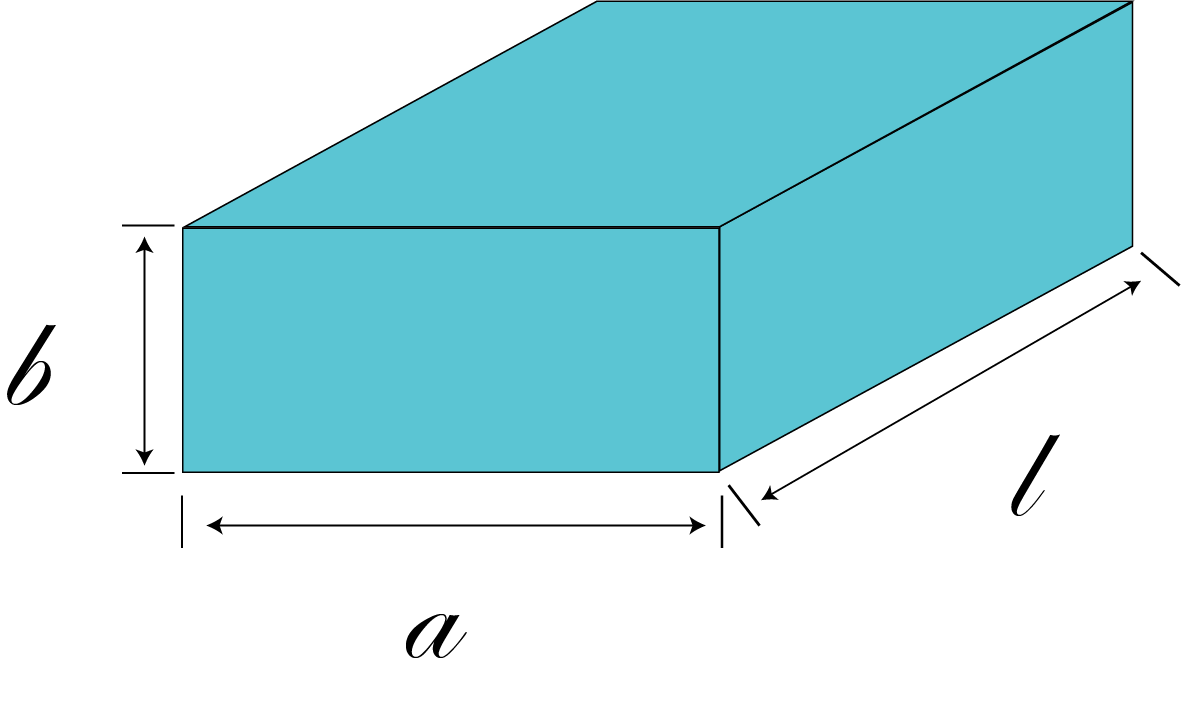
\includegraphics[width=5cm]{./image/空洞共振器.png}
    \caption{方形空洞共振器}
    \label{fig:Cavity}
  \end{center}
\end{figure}

\subsection{誘電体挿入時の共振周波数変化}

\vspace{10 mm}

\begin{figure}[h]
  \begin{center}
    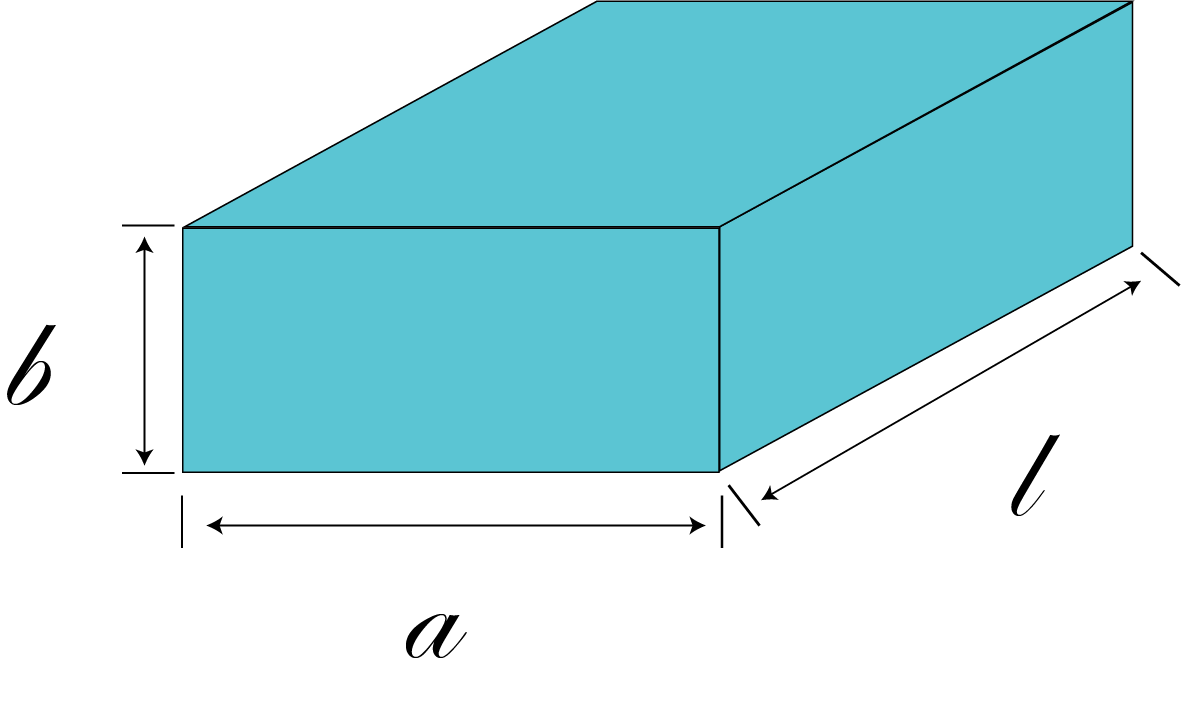
\includegraphics[width=5cm]{./image/空洞共振器.png}
    \caption{方形空洞共振器}
    \label{fig:Cavity}
  \end{center}
\end{figure}

\subsection{考察}
